\documentclass[a4paper, 11pt, twoside]{article}
\usepackage{amssymb}
\usepackage{amsmath}
\usepackage{graphicx}
\begin{document}
\title{STAT6038 week 6 lecture 17}
\author{R. Q.}
\date{2017-03-30}

\maketitle

\paragraph{Outlier and Influence Measures}\ \\

Main residual plots

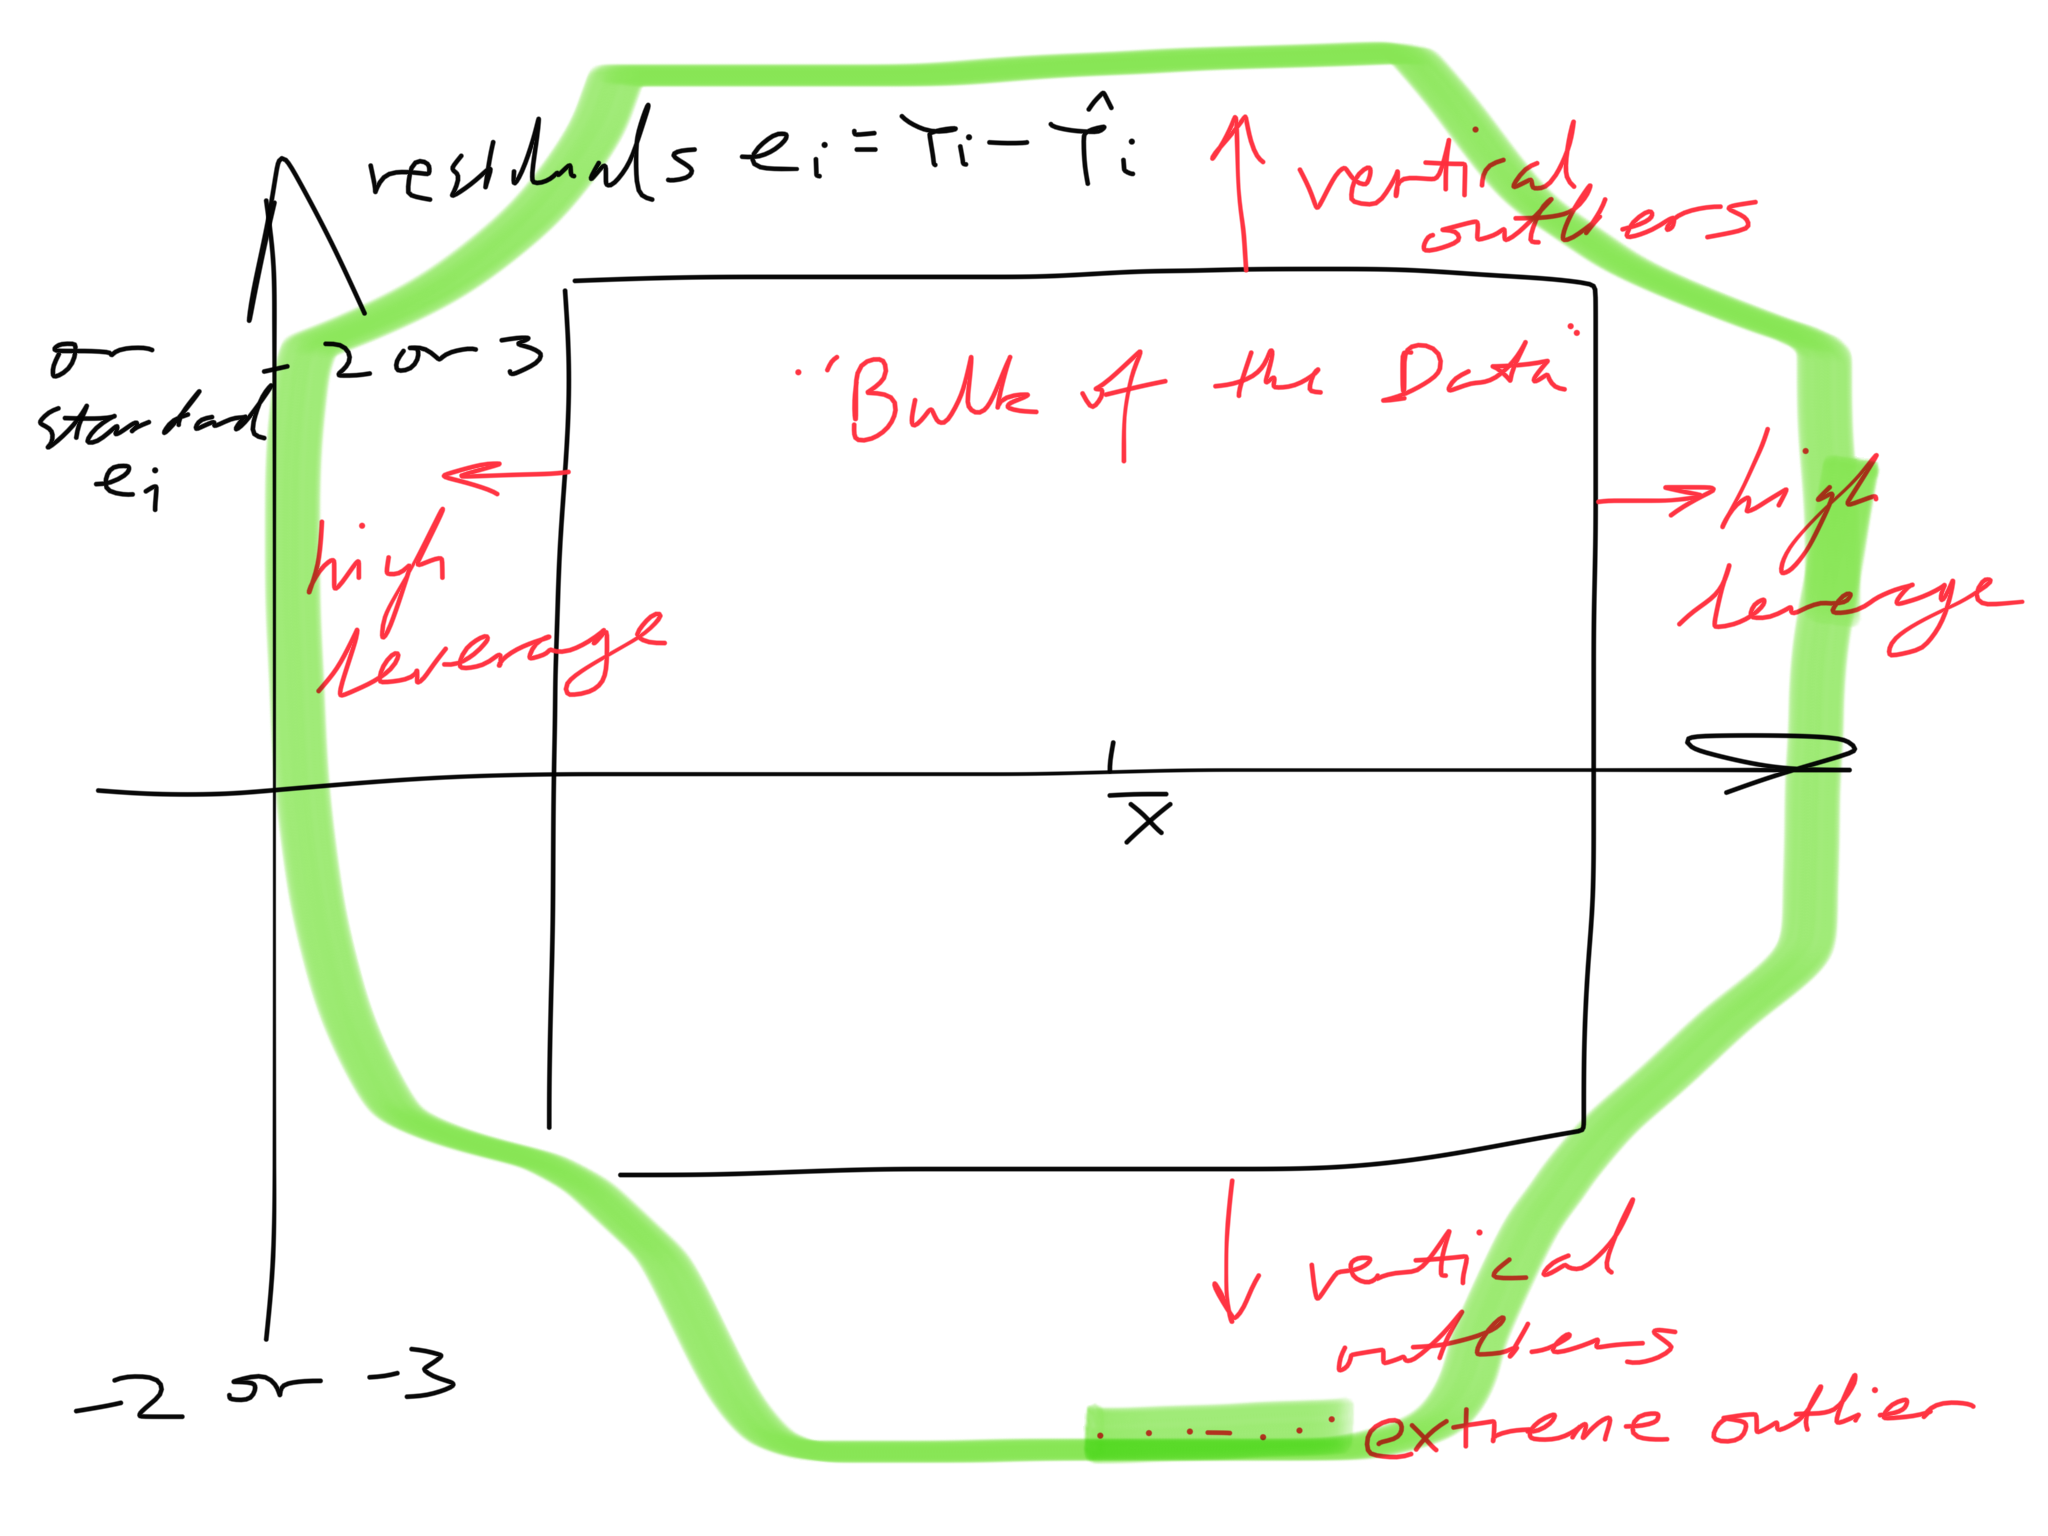
\includegraphics[width=\textwidth]{main-residual}

It is called the "region of possible problems" or "discordant observations"\\

Some of the literature bumps(?) all the ``discordant observations`` as ``outliers``, but outliers are really observations that are away from the bulk of data in some sense, i.e. there is a noticeable gap.\\

Cook \& Weisberg Technometrics: ``Outlier ....... s``\\

Other literature will talk about ``discordant observations`` as a general term \& distinguish between 

\begin{itemize}
	\item ``vertical`` outliers
	\item high leverage points
	\item highly influential observations (a bit of ``both`` of the previous)\\
\end{itemize}

\textbf{A good measure of ``both`` is a relatively Cook's Distance (we will discuss the formula later).}\\

\end{document}